\documentclass[tikz,border=10pt]{standalone}
\usepackage{amsmath}
\usepackage{tikz}
\usetikzlibrary{arrows.meta, positioning, calc, shapes.geometric}

\begin{document}
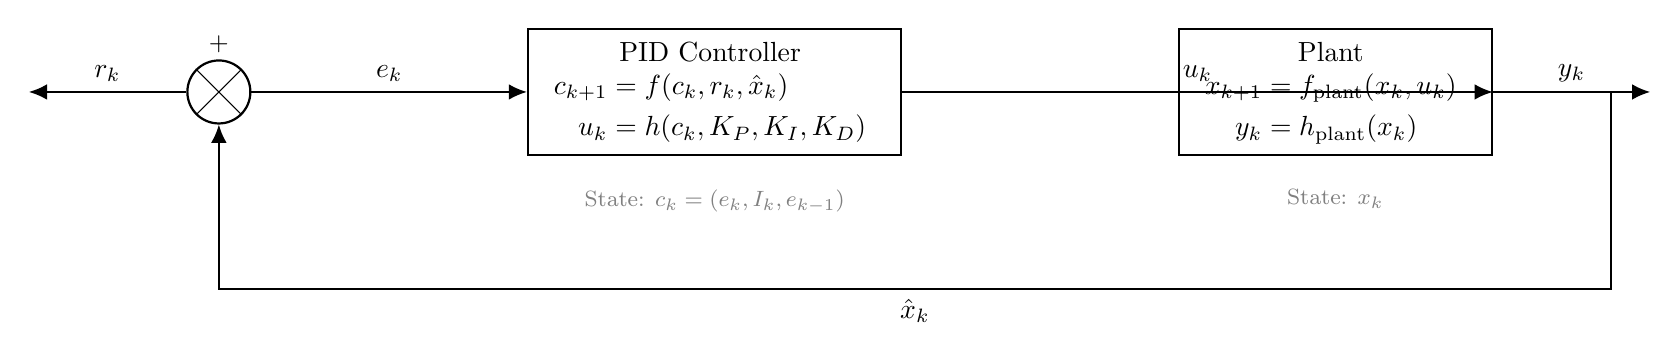
\begin{tikzpicture}[
  block/.style = {draw, thick, minimum height=3em, minimum width=6em, align=center},
  sum/.style = {draw, circle, thick, minimum size=0.8cm},
  arrow/.style = {thick, -{Latex[width=2mm]}},
  node distance=2.5cm and 3.5cm
]

  % Summing junction (error computation)
  \node[sum] (sum) at (0,0) {};
  \draw (sum.north east) -- (sum.south west);
  \draw (sum.north west) -- (sum.south east);
  \node at (sum.north) [above, inner sep=2pt] {\small $+$};
  \node at (sum.west) [left, inner sep=2pt] {\small $-$};

  % PID Controller block
  \node[block, right=of sum] (pid) {
    \begin{tabular}{c}
      PID Controller\\
      $\begin{aligned}
        c_{k+1} &= f(c_k, r_k, \hat{x}_k) \\
        u_k &= h(c_k, K_P, K_I, K_D)
      \end{aligned}$
    \end{tabular}
  };

  % Plant block
  \node[block, right=of pid] (plant) {
    \begin{tabular}{c}
      Plant\\
      $\begin{aligned}
        x_{k+1} &= f_{\text{plant}}(x_k, u_k) \\
        y_k &= h_{\text{plant}}(x_k)
      \end{aligned}$
    \end{tabular}
  };

  % Reference input
  \draw[arrow] (sum.west) -- ++(-2,0) node[midway, above] {$r_k$};

  % Error to PID
  \draw[arrow] (sum.east) -- node[above] {$e_k$} (pid.west);

  % PID to plant
  \draw[arrow] (pid.east) -- node[above] {$u_k$} (plant.east);

  % Plant output
  \draw[arrow] (plant.east) -- ++(2,0) node[midway, above] {$y_k$};

  % Feedback path
  \coordinate (feedback) at ($(plant.east) + (1.5,0)$);
  \draw[arrow] (feedback) |- ++(0,-2.5) -| node[pos=0.25, below] {$\hat{x}_k$} (sum.south);

  % Labels below blocks
  \node[below=0.3cm of pid, font=\footnotesize, text=gray] {State: $c_k = (e_k, I_k, e_{k-1})$};
  \node[below=0.3cm of plant, font=\footnotesize, text=gray] {State: $x_k$};

\end{tikzpicture}
\end{document}
